\documentclass[journal]{vgtc}                % final (journal style)
%\documentclass[review,journal]{vgtc}         % review (journal style)
%\documentclass[widereview]{vgtc}             % wide-spaced review
%\documentclass[preprint,journal]{vgtc}       % preprint (journal style)
%\documentclass[electronic,journal]{vgtc}     % electronic version, journal

%% Uncomment one of the lines above depending on where your paper is
%% in the conference process. ``review'' and ``widereview'' are for review
%% submission, ``preprint'' is for pre-publication, and the final version
%% doesn't use a specific qualifier. Further, ``electronic'' includes
%% hyperreferences for more convenient online viewing.

%% Please use one of the ``review'' options in combination with the
%% assigned online id (see below) ONLY if your paper uses a double blind
%% review process. Some conferences, like IEEE Vis and InfoVis, have NOT
%% in the past.

%% Please note that the use of figures other than the optional teaser is not permitted on the first page
%% of the journal version.  Figures should begin on the second page and be
%% in CMYK or Grey scale format, otherwise, colour shifting may occur
%% during the printing process.  Papers submitted with figures other than the optional teaser on the
%% first page will be refused.

%% These three lines bring in essential packages: ``mathptmx'' for Type 1
%% typefaces, ``graphicx'' for inclusion of EPS figures. and ``times''
%% for proper handling of the times font family.
\usepackage{amssymb} 
\usepackage{amsmath}
\usepackage{mathptmx}
\usepackage{graphicx}
\usepackage{times}
\usepackage{comment}

%% We encourage the use of mathptmx for consistent usage of times font
%% throughout the proceedings. However, if you encounter conflicts
%% with other math-related packages, you may want to disable it.

%% This turns references into clickable hyperlinks.
\usepackage[bookmarks,backref=section,linkcolor=black]{hyperref} %,colorlinks
\hypersetup{
  pdfauthor = {Biswarup Mukherjee},
  pdftitle = {Metaballs 2016, DeNovi et al.},
  pdfsubject = {},
  pdfkeywords = {},
  colorlinks=true,
  linkcolor= black,
  citecolor= black,
  pageanchor=true,
  urlcolor = black,
  plainpages = false,
  linktocpage
}

%% If you are submitting a paper to a conference for review with a double
%% blind reviewing process, please replace the value ``0'' below with your
%% OnlineID. Otherwise, you may safely leave it at ``0''.
\onlineid{0}

%% declare the category of your paper, only shown in review mode
\vgtccategory{Research}

%% allow for this line if you want the electronic option to work properly
\vgtcinsertpkg

%% In preprint mode you may define your own headline.
%\preprinttext{To appear in an IEEE VGTC sponsored conference.}

%% Paper title.

\title{Metaballs Approach to Cut and Fracture Simulation in Virtual Surgery  }

%% This is how authors are specified in the journal style

%% indicate IEEE Member or Student Member in form indicated below
\author{Gianluca De Novi \textit{Member, IEEE}, Biswarup Mukherjee, \textit{Member, IEEE}, and Mark P. Ottensmeyer}
\authorfooter{
%% insert punctuation at end of each item
\item
 Gianluca De Novi, Biswarup Mukherjee and Mark P. Ottensmeyer are with the Simulation Group at Massachusetts General Hospital and Harvard Medical School, USA. E-mail:gdenovi@seas.harvard.edu.
}

%other entries to be set up for journal
\shortauthortitle{Biv \MakeLowercase{\textit{et al.}}: Global Illumination for Fun and Profit}
%\shortauthortitle{Firstauthor \MakeLowercase{\textit{et al.}}: Paper Title}

%% Abstract section.
\abstract{Duis autem vel eum iriure dolor in hendrerit in vulputate
velit esse molestie consequat, vel illum dolore eu feugiat nulla
facilisis at vero eros et accumsan et iusto odio dignissim qui blandit
praesent luptatum zzril delenit augue duis dolore te feugait nulla
facilisi. Lorem ipsum dolor sit amet, consectetuer adipiscing elit,
sed diam nonummy nibh euismod tincidunt ut laoreet dolore magna
aliquam erat volutpat. Ut wisi enim ad minim veniam, quis nostrud exerci tation ullamcorper
suscipit lobortis nisl ut aliquip ex ea commodo consequat. Duis autem
vel eum iriure dolor in hendrerit in vulputate velit esse molestie
consequat, vel illum dolore eu feugiat nulla facilisis at vero eros et
accumsan et iusto odio dignissim qui blandit praesent luptatum zzril
delenit augue duis dolore te feugait nulla facilisi.
} % end of abstract

%% Keywords that describe your work. Will show as 'Index Terms' in journal
%% please capitalize first letter and insert punctuation after last keyword
\keywords{Metaballs, Cut simulation, fracture simulation}

%% ACM Computing Classification System (CCS). 
%% See <http://www.acm.org/class/1998/> for details.
%% The ``\CCScat'' command takes four arguments.

\CCScatlist{ % not used in journal version
 \CCScat{K.6.1}{Management of Computing and Information Systems}%
{Project and People Management}{Life Cycle};
 \CCScat{K.7.m}{The Computing Profession}{Miscellaneous}{Ethics}
}



%% Uncomment below to disable the manuscript note
\renewcommand{\manuscriptnotetxt}{}

%% Copyright space is enabled by default as required by guidelines.
%% It is disabled by the 'review' option or via the following command:
% \nocopyrightspace

%%%%%%%%%%%%%%%%%%%%%%%%%%%%%%%%%%%%%%%%%%%%%%%%%%%%%%%%%%%%%%%%
%%%%%%%%%%%%%%%%%%%%%% START OF THE PAPER %%%%%%%%%%%%%%%%%%%%%%
%%%%%%%%%%%%%%%%%%%%%%%%%%%%%%%%%%%%%%%%%%%%%%%%%%%%%%%%%%%%%%%%

\begin{document}

%% The ``\maketitle'' command must be the first command after the
%% ``\begin{document}'' command. It prepares and prints the title block.

%% the only exception to this rule is the \firstsection command
\firstsection{Introduction}

\maketitle

In the last thirty years, minimally invasive surgery (MIS) has been improving patient safety and reducing the time of permanence within hospitals consistently ~\cite{mishistory1}. 
The MIS approach to surgery allows the surgeon to perform a classic operation (open surgery) avoiding opening
the patient body, but just using few small holes where he/she can introduce particular
surgical tools and, in some cases, a camera too. There are many different MIS
surgical practices but the principal two categories are the laparoscopy (thorax and
abdomen) and catheter-based procedures. The first typology of operations requires
the use of a camera in order to see the surgical operation field and to control the
surgical tools. The use of MIS tools requires very strong manual skills. As a result,
surgeons need to spend a significant amount of time improving their skills surgical
through the use of trainers. Usually, surgeons need to use trainers for new surgical
procedures or for new surgical tools. There are different kind of trainers used to
improve the surgeons skills:  


The use of cadavers and animals raise ethical issues and are allowed in only a few
countries. Often, their use requires special permissions. One issue with this method
is represented by the fact that the animal should be alive because the behavior of the
in-vivo tissues is completely different from the dead tissues. The trainer box
represents an acceptable solution. It requires the use of a box in order to simulate the
abdomen or the thorax of the patient and it includes the use of latex/silicon organ
models. The trainer box results in an expensive educational tool because, after few
simulations, the silicon models need to be replaced and the behavior of those models
is not realistic.



\section{Soft-tissue model using metaballs}

\begin{figure}[!b]
    \centering
    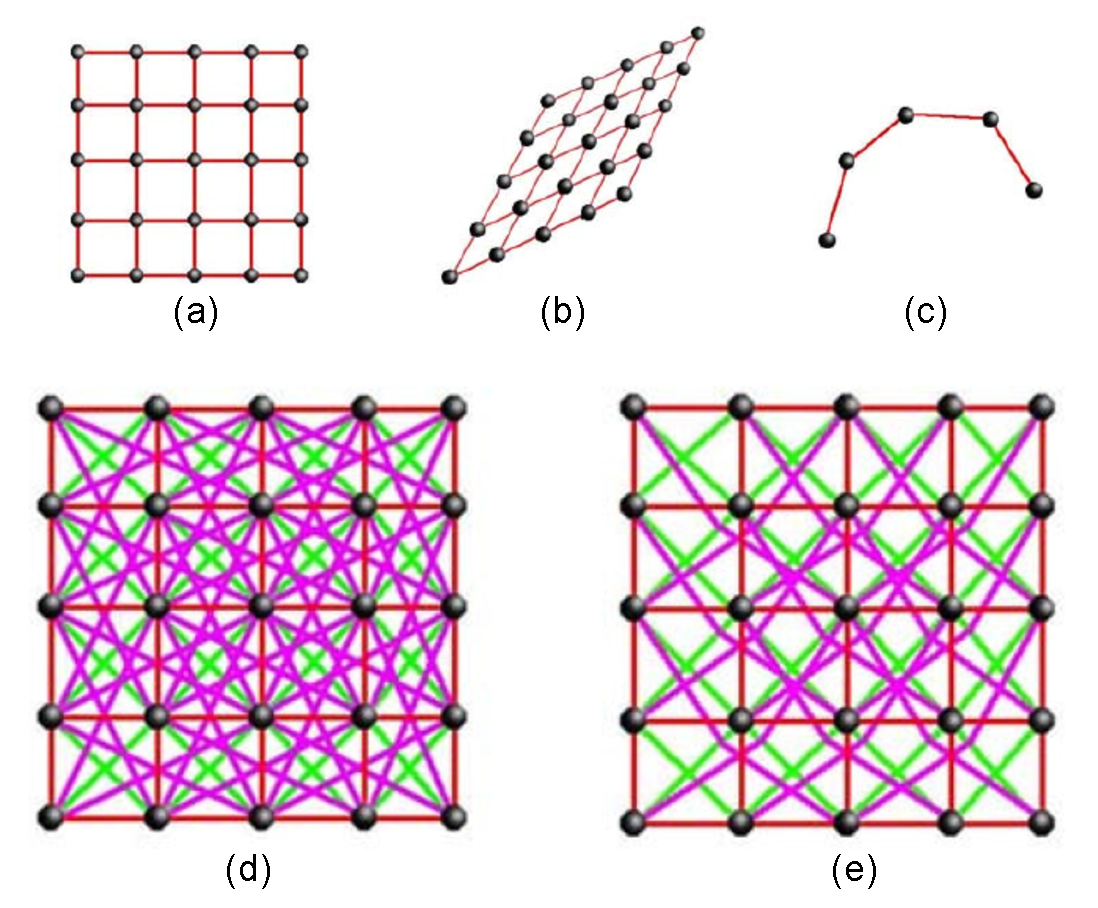
\includegraphics[width=0.45\textwidth]{Figures/Fig1.eps}
    \caption{Caption}
    \label{fig:fig1}
\end{figure}
\textbf{From chapter 3}

In order to simulate a dense soft tissue organ, it is indispensable to create a tridimensional mesh of particles and visco-elastic links.
Using the metaballs approach, the creation of the tridimensional mesh can be
difficult when the resolution of the sphere tree is low. The first topic that needs to be
discussed is the strategy used for an automatic network creation starting from the
sphere tree. As we know, the behavior of a soft tissue model can be strongly
influenced by the connection topology used for the tridimensional mesh \textbf{Refer}. In some
cases, a wrong connection topology could create an odd behavior that does not match with the desired (real) one.




If, in an elastic cloth simulation, a mesh model is used as shown in figure 4.1a, we
will obtain two wrong behavior non-elastic deformations) that do not match with the
behavior of a real elastic cloth. In figure 4.1.b, the elastic cloth collapses in a single
segment without deforming any link (the deformation is stable); in the figure 4.1c,
the elastic cloth can be deformed also without an elastic deformation. Adopting a
connection scheme, as shown in figure 4.2a using cross-links (green and violet links)
and an optimized version in 4.2b, is a possible solution to the non-elastic
deformations for the elastic cloth simulation.

\begin{figure}[!t]
    \centering
    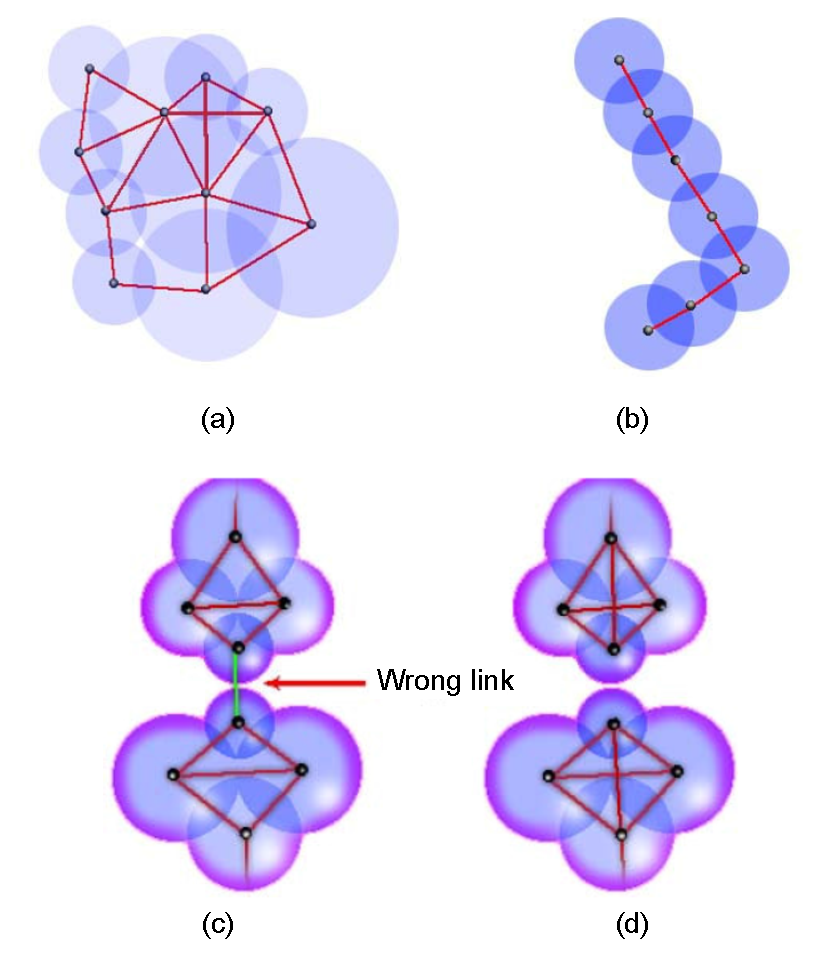
\includegraphics[width=0.45\textwidth]{Figures/Fig2.eps}
    \caption{Caption}
    \label{fig:fig2}
\end{figure}

For tridimensional meshes, the topology connection requires a complex building
process. In our case, after the conversion from volumetric model (or polygonal
model) to a sphere tree, we obtain only a set of spheres. A first approach to create a
tridimensional mesh on the sphere tree could be to connect, with visco-elastic links,
all the overlapped spheres (neighbor connection strategy - figure 4.3a).

The neighbor connection strategy works well and is easy to implement, but it is not
able to avoid non-elastic deformation (figure 4.3b). Usually, the non-elastic
deformation is obtained for all spheres connected with less than three links (not
aligned). It is possible to setup a proper algorithm able to recognize if a specific
sphere is connected in the right way with the neighboring spheres, and to connect it
with the closest sphere in case there are less than three connection links. In general,
this approach needs to be integrated with a manual procedure, because it still
presents some problems, such as the ghost links as shown in figure 4.4a. During the
creation of the mesh and the creation of the correct minimal number of connections
for each particle, through choosing the closest particles, it is possible to create ghost
links, connecting a specific particle with another one that is outside the local body
surface.

As discussed in chapter one, the avoidance of the ghost link is an expensive task for
the fracture simulation; however, in this case, we need to perform the mesh
generation task only one time, before to start the simulation. As a result, it is
possible to implement a proper algorithm able to recognize and fix ghost links
through creating a new proper connection scheme. During mesh generation, there are
also other situations where the neighbor approach does not produce the best
connection topology. For a right connection scheme, all the links (the first three) for
each particle should be connected with other three non-coplanar particles, creating a
tetrahedron (figure 4.5a). If the three closest particles are coplanar with the first one,
the connection topology does not work well because the tridimensional deformations
cannot have the same elastic behavior on a direction normal to the particles plane.
All forces applied in that direction will not be correctly balanced by the mesh (figure
4.5b).

Nevertheless, the opportunity to create tetrahedral connections is not always
possible. In some specific cases, a coplanar connection is the only possible scheme.
If we consider, for example, a minimal blobby model (using a minimal sphere set)
for the intestines, the only possibility is to use a segment of spheres. In this last case
all spheres present two connections, except the first and the last sphere (figure 4.3b);
the chain connection scheme does not work because it allows non-elastic
deformation. In this case, the neighbor strategy produced a satisfactory result,
introducing cross-links (figure 4.5).

Through the use of cross-links in a chain, it is possible to avoid the non-elastic
deformation. This occurs because when trying to bend a short section of the chain,
the cross-links create a resistance force to balance the bending force.

An interesting property of the sphere tree approximation using the [14] is that the
resolution of the sphere tree grows close the edges, increasing the number of spheres
and reducing the ray in order to fit the original model in the best way. As told in
chapter two, the blobby approach works well for the surgical simulations, because,
by having rounded organ models, the number of spheres tends to be low. The high
sphere tree resolution on the edges allows the simulation to indirectly describe all
parts of the models where it is easier to have a deformation (more deformable areas),
providing a better accuracy (figure 4.7). In some cases in the educational surgery
simulations, the main goal is not the accuracy of the model but the simulation of a
realistic behavior. In those cases, the neighbor connection strategy extended with the non-elastic deformation avoidance is not the best approach, because it is not able to assure a correct elastic behavior. Consider a semi-rigid chain of metaballs: using the
neighbor strategy it is not possible to achieve realistic elastic behavior, because the
chain is not able to react to the orthogonal forces and the result is the bending of the
chain. A possible solution is represented by the possibility to use a Bounding
Connection Set that is an external set of links connected between each particle and
the edge of the model-bounding box (figure 4.8).

Using the Bounding Connection Set, it is possible to keep a reasonable stiffness for
shapes thin and long. During the simulation flow, the bounding box vertices will not
be considered as particles; this means that all the link force will load on the
connected particle. Also, the bounding box vertices will not be considered for
collision detection. Instead, they will be considered as “ghost particles”. The
bounding box does not have mass. There are different types of connection strategies
and, as mentioned at the beginning of this section, the results in terms of
computational performances and in terms of behavior depends from the right choice
of the kind of model and when considering the required dynamics. By setting all
tissue parameters inside the mesh and deciding on the best connection strategy, the
final behavior during the simulation should be able to satisfy the initial requirements
creating bubble deformation objects (figure 4.9).

\subsection{Blobby versus FEM mesh}

As shown before, using metaballs and the described procedure, it is possible to
generate a tridimensional model able to simulate a soft tissue volume. In regards to
the FEM (finite element Model), there are some differences. A first difference is that
in the FEM (for example meshes of tetrahedrons), the finite element is a tetrahedron;
each tetrahedron can be deformed by simply deforming its links. Using the blobby
meshes, the “finite element” is just a sphere that cannot be deformed, and the model
deformation is solely performed on the mesh links. This last feature means that there
is a limit for the model deformation, and over this limit it is not possible to deform
the body, introducing a behavior not coherent with the reality. The normal FEM
model, under a large force, can collapse to a zero thickness model, allowing another
non-realistic situation.

Another important limitation of the blobby meshes is that by using a MAA sphere
tree, the resultant model does not allow some types of deformations (i.e. local
deformations) due the low resolution of the dynamic mesh (figure 4.15a, 4.15b).

From a different point of view, the reduction of the mesh resolution determines a
growth of the computing performances, and it could be an important feature for all
simulation applications where accuracy is not the most important feature.

\section{Local Interaction Model for Metaball based Soft-tissue}

As explained in the previous chapter, the metaballs approach to the soft tissue
presents some limitations using the MAA for the creation of the sphere tree. Through
obtaining a low resolution mesh, it is possible to keep a global behavior, but it is not
possible to obtain local deformations. During a surgery simulation, the global model
behavior is very important, but the local deformations are important too: they
increase the realism of the interaction and, in some cases, it is indispensible for
particular kinds of surgical tools. The local deformations, however, are usually
hidden behind the surgical tool and it is possible to recognize them just in proximity
to the surgical tool. The fact that the local deformations are usually hidden means their accuracy can be unimportant in terms of visual perception. Starting from this last consideration, we can expect to introduce a new approximation about the body
deformations that is not coherent with reality but is acceptable in terms of
computational cost reduction for the simulation. The introduced assumption is to
consider the body deformations as a contribute of two different kinds of deformation
(Figure 5.1):
\begin{itemize}
\item Local deformation.
\item Global deformation.
\end{itemize}
By expecting to split the deformations in two different contributes, it is possible to
keep the global deformation provided by the low resolution mesh and it is possible to
simulate “fake” local deformations using a trick.

As mentioned in the chapter two, when working with metaballs it is possible to use
metaballs with different signs, and the effect on the iso-surface is a local deformation
(using a metaball of a proper ray). The local deformation is exactly what we need in
order to simulate the interaction with a surgical tool (figure 5.2). Assuming the use of
positive field generators for the organ model, the only actions needed is to associate a
negative metaball to the surgical tool. When the surgical tool touches the iso-surface
it will look deformed, simulating a local deformation with an acceptable realism. Considering a single point tool model, the local surface deformation that we can obtain has a concave profile, completely different from the real deformation that we
should obtain in a real case (Figure 5.3a and 5.3b).

Adopting a multipoint tool model, the local deformation shape can be improved; in
fact, the local deformation will copy the exact shape of the surgical tool (Figure 5.4). The proposed local deformation technique can simulate local deformations only from a visual point of view. In order to work in an accurate way, it needs to be supported
by a physic point of view with the intention of generating feedback forces. By using
the proposed approach, switching the tool’s particle signs, and modeling the surgical
tool with a proper particle set, it is possible to simulate very complicated local
deformations, to improve the realism of the simulation, and to keep the simulation
operating at optimal speed.

After we improved the local deformation between the surgical tool and the organ
model, it is indispensible to define a collision detection model optimized for the
metaballs approach and able to exploit all features discussed in the past chapters. In
general, a blobby model is just a way to generate a potential field and an iso-surface
with a desired shape. Inside the iso-surface, the field intensity will be higher than
outside, defining a scalar collision detection function implicitly able to evaluate if a
collision occurs in a generic point $p \in \mathbb{R}^{3}$ is inside as:

\[
 \sigma(p) = 
  \begin{cases} 
   1    &       \text{if } \Phi (p) > \tau\\
   0    &       \text{if } \Phi (p) = \tau\\
  -1    &       \text{if } \Phi (p) < \tau\\
  \end{cases}
\]

where $\Phi (p)$ is the field function that is able to describe the field intensity in a generic point, $p$, such that,

\begin{equation}
\Phi(p) = \sum_{i=0}^{n} f_{i} (p)
\end{equation}

$f_{i}(p)$ is the field function for the metaball $i$ at the point $p$. In this manner, it is possible to understand the generic point $p$ is inside ($\sigma (p) =1$) or outside ($\sigma (p) = -1$) the volume, or if it is on the iso-surface ($\sigma(p) = 0$). Moreover, it is also possible to approximate the minimal distance $\delta \tau$ between the point $p$ with $\phi(p)= \epsilon$ and the iso-surface calculating.

\begin{equation}
\delta \tau (\epsilon) \approx \left| f^{-1} (\epsilon) - f^{-1}(\tau) \right| = \left| \sqrt[m]{\frac{I_{c}}{\epsilon}-\frac{I_{c}}{\tau}} \right|
\end{equation}

where $I_{c}$ is the intesity of the closest field generator. The approximation
introduces an error on the minimal distance computation, but by using a high value
for $m$, it can be neglected. This last value could be used, in case of haptic rendering,
for the interaction force modulation, approximating the surgical tool such as a point.
In case a collision occurs, i.e. $\sigma(p) = 1$ 
, it is possible to define a local reaction force
vector $f_{r}$, with amplitude given by the Hook Law as:

\begin{equation}
\left|| f_{r}(p) \right|| = k \delta _{\tau}(\epsilon)
\end{equation}
 
where $k$ is related to the local stiffness of te object and direction as given by equation 


\begin{equation}
\hat{f}_{r}(p) = \frac{\sum_{i=0}^{n} \left[\frac{p-c_{i}}{\left|p-c_{i}\right|}\right]}{\left| \sum_{i=0}^{n} \left[\frac{p-c_{i}}{\left| p-c_{i}\right|}\right]\right|}
\end{equation}

that follows the field anti-gradient $-\nabla \phi (p)$ direction. This force can be used for
haptic rendering purposes, e.g. for the god object method, \textbf{Refer here}. In terms of collision
response, it is possible to use the same approach discussed in the section 3.2,
modeling the collision as a soft collision, distributing the contact forces to the
surgical tool and on the soft tissue.

Moreover, the surface friction can also be modeled on the iso-surface by means of
classic formulations, considering $f_{t}$ and $f_{n}$, the tangential and normal component to
the surface of the force vector $f_{r}$. For example, a static condition is obtained if

\begin{equation}
\left|f_{t}\right| \le \mu _{s} \left|f_{n}\right|
\end{equation}

while a viscous friction can be computed as 

\begin{equation}
\left|f_{d}\right| \le \mu _{d} \left|f_{n}\right| \hat{v}_{t}
\end{equation}

where $\mu _{s}$ and $\mu _{d}$ represent the static and dynamic friction coefficients and $\hat{v}_{t}$ is the direction of the tangential velocity. From the algorithm point of view, the collision detection can
be written as in the source 5.1. When looking at the source code, it is evident that by
using the metaballs approach, the collision detection is very fast because it does not
need to perform complicated polygons intersections; the collision detection requires
only the evaluation of a field function in a specific point of the space, with a linear
complexity. From a computational point of view, this last result is very important,
because using the classic approach (meshes of FEM), the collision detection was
very expensive and tricky to implement. At this point, the principal advantages
achieved using the metaballs approach can be represented by the possibility of
reducing the mesh complexity, keeping the local deformation and a very fast
collision detection; these are two important results that save a considerable amount
of time that can be spent on the execution of other tasks such as improving the speed
and the complexity of the simulation. The source code 5.1 does not implement any
optimization, but in the case of complex geometries, with a big number of metaballs
(i.e. n > 50k), a spatial subdivision could be implemented in order to improve the
computational performances. It is necessary to remark that with more than 50k
metaballs it is possible to create very complex geometries.

\subsection{Multi-body Interactions}
There are several advantages obtained through the use of the metaballs approach; it is
possible to save a great deal of computational power that could be spent improving
the realism of the surgical scene. A first important feature that can be implemented is
the multi-body simulation, allowing the simulation to manage multiple soft/hard
bodies. The multi-body extension is based on the same technique used for the local
interaction: using different signs for the local deformation and a soft particle
collision response. The first difference, however, is that by having more than two
bodies, the use of two signs is not a possible solution, so the multi-body extension
requires the use of a body ID for each metaball. This is necessary to determine if a
specific metaball belongs to a specific body. By using the body ID, it is possible to
sum the contribute of all metaballs with the same ID and to subtract the contribute
for the others.

Through extending the simulation with the multi-body feature, the field function and
the collision detection changes as shown in the source 5.2 (all modifications are in
red). The last modification for the collision detection slightly increase the complexity
when a single body was just linearly dependant to $n$ (number of metaballs) to $n \times m $ where $m$ is the number of bodies inside the simulation. When using two metaballs with different ID’s, the contact should looks like in Figure
5.5. Another important modification is for the drawing task. This needs to be
modified because in the multi-body case, each body should be drawn separately,
spending more time extracting each body surface separately. In order to improve the
multi-body collision detection and response in a scene with a large number of
metaballs, the octree space partitioning represents a good solution. A single metaball
as field generator generates an infinite field from the source position; knowing this,
before using an octree, it is indispensible to define a cutoff threshold in order to
identify where the field should be approximate to zero. In this way, it is possible to
say that each metaball field has effect on a specific distance and over that distance
the field effect can be ignored.

\subsection{Multilayered Surfaces}

Another possible improvement that could easily achieved for the interaction model is
the multilayered model. The human body is made of organs (e.g. muscles)
overlapped with bones or other tissues with different visco-elastic properties. In the
multilayer case, the local interaction force $f_{r}$ needs to be calculated considering all
the contributions of the different layers. With the metaballs approach, the multi-layer
extension can be easily obtained by considering more threshold values (or using
particular rules in the field generation algorithm, but in this thesis we only consider
the multi-threshold case for simplicity). If we consider $n$ iso-surfaces, we can define
the local interaction force as obtained by $n$ springs, each of them with different
properties, connected in series, see figure. 5.6.

As an example, consider two surfaces $S_{1}$ and $S_{2}$  of thickness $L_{1}$ and $L_{2}$
and stiffness constants $k_{1}$ and $k_{2}$ respectively (in this case, linear spring are used for simplicity, but
more complex functions could be considered as well). If a deformation $\Delta x$ is applied
on the external organ surface, the deformation on each spring can be computed from:

\begin{equation}
\begin{split}
\Delta x_{1} & = \frac{k_{2}}{k_{1} + k_{2}} \Delta x \\
\Delta x_{2} & = \frac{k_{1}}{k_{1} + k_{2}} \Delta x 
\end{split}
\end{equation}

considering the equivalent $k_{eq}$

\begin{equation}
k_{eq} = \frac{k_{1}k_{2}}{k_{1} + k_{2}}
\end{equation}

the amplitude of the resultant elastic force is

\begin{equation}
\left| f_{r} \right| = k_{eq} \Delta x = k_{eq}(\Delta x_{1} + \Delta x_{2})
\end{equation}

while its direction is the same as $\hat{f}_{r}(p)$ for the haptic tool. The computed force is projected also on the closer particles and then to their visco-elastic links,
resulting in a deformation of the global model, figure 5.7. The global deformation
can be obtained only through a local interaction and deformation; the feedback force
provided to the haptic tool will be the sum of two contributes: a local interaction force and a global deformation force that will be computed as the resultant force
applied by the tridimensional mesh on the touched particles.

\section{Fracture Simulation in Metaball Based Soft-tissue}

Fractures simulation is a task that is not often performed during operations, because the usual way to remove pieces of tissue is using cutting tools in order to avoid tissue damage. Fracture simulation is performed, however, where it is not possible to directly cut the tissue. For the metaballs approach, the adopted fracture model can be exactly the same as used for the classic FEM meshes, working directly on the connection links. \textbf{As mentioned in the chapter four}, each link has a breaking threshold that is used in order to recognize if the link should be broken during the deformation. With respect to the FEM model, in the fracture simulation, using the breaking threshold works better because when the links are broken and the volume is subdivided; it is not necessary to rebuild the fracture internal surface, because the surface will automatically generated during the iso-surface extraction with marching cube algorithm.

It is possible to perform the fracture simulation saving precious time that can be
spent on improving other elements. Unfortunately, when using the same technique
for the fracture simulation, it is not possible to avoid ghost links (figure 6.2). If the
model geometry is not extremely complex, it is possible to implement a proper
algorithm for ghost link avoidance. A possible limitation for the fracture simulation
using metaballs is the extremely rounded aspect of the fractures; this does not match with reality that usually is not rounded and looks more similar to the FEM fracture simulation.

This fact happens because if the broken link connects two big metaballs, the fracture
will have as profile, the metaball profile, and will look rounded. In the case of FEM
fractures, the fracture follows the tetrahedral mesh and the fracture assumes an
irregular aspect and severs with very clear edges. Usually, the fractures in surgery are
applied on small pieces of tissues, then under this last hypothesis the rounded aspect
could be acceptable, considering the other advantages achieved using this method. In
terms of algorithm complexity, the fracture simulation could be implemented as
shown in the source 6.1 (C++ code snippet for the link computation block, see figure
1.4).



\section{Cut Simulation}

The cutting simulation is still an open issue today in the surgery simulation field
because is a very expensive and complex task. In the first chapter, there is a brief
discussion about this topic and an introduction on the related problems. Usually,
using the classic approaches, it was possible to perform cuts only on small portions of the scene, in order to reduce the complexity and the computational costs. Using the metaballs approach, the complexity of the cuttings simulation is strongly reduced, offering the possibility to perform cuts everywhere inside the surgical scene.

The first difference between the metaballs approach and FEM is that, in FEM, the cut
is performed on the mesh element (tetrahedron or different one), but in the metaballs
case, it is performed on the sphere, just because in this case the sphere is the minimal
volume element. The cut on the sphere is performed by recursively splitting the
sphere into a pattern of sub-spheres (reducing the sphere size). In case the spheres are
of a specific smaller size, the sphere is simply removed. As an example, using a 2D
version of this algorithm, we can assume to have a circles pattern (2D version of the
spheres pattern) like the pattern in figure 6.3.

When a circle that is greater than a specific size is touched by a surgical tool, the
circle is replaced recursively by a circles pattern with a proper size (the pattern will
be contained inside the starting sphere, figure 6.4a, 6.4b, 6.4c, 6.4d); if the circle is
smaller than the minimum size, the sphere is deleted (figure 6.4e).

Applying the splitting technique on a more complex soft tissue model, under the
gravity effect, the cut can be performed as shown in figure 6.5. Extending the model to the tridimensional case the spheres pattern could be as in figure 6.6. The metaball split is not enough for the cutting simulation, because the replaced metaball was connected with visco-elastic links to other metaballs (see figure 6.5).

After the split, it is necessary to connect the new spheres pattern to the existing
metaballs mesh. The new spheres pattern will come already connected internally and
each sub-sphere will be connected with the external spheres previously connected
with the replaced one (figure 6.7).

Remarking in few words the cutting algorithm can be expressed in few rules:

\begin{itemize}
\item Each sphere touched by the cutting tool will be replaced by a specific pattern
internally connected in a specific way.
\item Each sphere of the pattern will be connected with all external spheres
previously connected with the replaced sphere and the elasticity constant will
be subdivided for each new link.
\item The mass of a replaced sphere will be subdivided between all new spheres.

\item The recursive splitting will be stopped on a minimum sphere size (minimum
ray); after that, each sphere and its link will be removed. 
 
\end{itemize}  

\subsection{Cutting Optimization}

The metaballs cutting, such as the FEM mesh cutting (using the tetrahedron
splitting), increases the mesh complexity for each metaball split. A first difference is
that a single metaball split increases the mesh complexity faster than the tetrahedron
split. For example, in the metaball split, using a six sphere set, the metaball number
is increased by five and the internal links number increases by fifteen plus five times
the number of external links (table 6.1).

Considering that when we split a metaball to simulate a cut, the old sphere is
removed and at least one sphere of the set is removed; the table for the cut become
such as the table 6.2.

Finally, the result is that for a single metaball connected with five external links a
single cut increase the metaballs by five and the links by thirty. At the second level
of cutting, each single sphere will be connected with four old internal links plus five
old external links, and then the complexity will grow quickly. A possible solution for
the proposed approach is to connect each external link after the sphere replacement,
not with all the new metaballs, but just with the closest one.

Adopting the proposed optimization, it is possible to reduce the complexity growth,
but this solution does not assure the non-elastic deformations avoidance. Another
possible solution could be to connect sequentially each external link with the closest
unconnected metaball. Even so, considering that the number of metaballs is very low,
thanks to the MAA, the complexity growth represents an unimportant problem
(usually < 10k for a complex surgical scene).
Usually after a cut, inside the mesh there may be residual metaballs, very small and
completely contained in other greater spheres connected with them; if so, it is
possible to remove those spheres. In order to understand if a sphere is contained
inside another one, a test must be performed considering the maximum link
extension before the breaking threshold (figure 6.9). If a sphere is contained inside
another one at the maximum link extension, that sphere will be removed from the
mesh, reducing the mesh complexity. This last test will be performed at runtime, on
only the new spheres introduced by the pattern used for the replacement; this is
inexpensive.

After this last discussion, it is easy to understand that the metaballs approach for the
soft tissue simulation can create a lot of advantages for surgery simulation
development, allowing the implementation of very sophisticated simulations,
keeping a low complexity and requiring a less expensive computational load.


\section{Conclusion}


%% if specified like this the section will be committed in review mode
\acknowledgments{
The authors wish to thank A, B, C. This work was supported in part by
a grant from XYZ.}

\bibliographystyle{abbrv}
%%use following if all content of bibtex file should be shown
%\nocite{*}
\bibliography{template}
\end{document}
